\section{Iterative Data Cleaning}\label{background}
This section introduces the problem of iterative data cleaning through an example application.

\subsection{Use Case: Dollars for Docs}\label{s:usecase}
ProPublica collected a dataset of corporate donations to doctors to analyze conflicts of interest~\cite{dollarsfordocsa}. 
Some of these donations are flagged as suspicious after careful manual review.
Suppose ProPublica wants to train a classification model to automate the flagging process in the future.
We collected the raw data and explored whether suspect donations could be predicted with an Support Vector Machine model.

However, this dataset has a number of inconsistencies.
On the ProPublica website \cite{dollarsfordocs}, they list numerous types of data problems that had to be cleaned before publishing the data (see Technical Report~\cite{activecleanarxiv}).
For example, company names were often inconsistently represented in the data, e.g., Pfizer Inc., Pfizer Incorporated, Pfizer.
A crucial data cleaning operation is to merge this inconsistency to a single value.
Duplicate representations could artificially reduce the correlation between certain companies and suspected contributions.
Furthermore, donation records were often inconsistently flagged, e.g. Suspiscious, Review, Disallowed.
Nearly 40,000 of the 250,000 records had some form of inconsistency.

When we analyzed this data, we found that the errors were not random and were correlated with the eventual prediction.
First, records that were suspicious were more likely to have an inconsistent flagging attribute.
Next, the names of the larger pharmaseutical companies were also more likely to have inconsistent names, and it turns out that these companies were also more likely to provide a flagged donation.
Without data cleaning, the true positive rate of an SVM model is only 66\%.
Applying the data cleaning to the entire dataset improved this rate to 97\% in the clean data (Section \ref{exp:dfd}).
This problem is typical of analysis scenarios based on observational data seen in finance, insurance, medicine, and investigative journalism.

For reference, the dataset has the following schema:
\begin{lstlisting}[mathescape,basicstyle={\small}]
Contribution(pi_specialty$\textrm{,}$ drug_name$\textrm{,}$ device_name$\textrm{,}$
$~~~~~~~~~~~~~~~~~~~~~~~~~~~~~~~$corporation$\textrm{,}$ amount$\textrm{,}$ dispute$\textrm{,}$ status)
\end{lstlisting}

\noindent\texttt{pi\_specialty} is a textual attribute describing the specialty of the doctor receiving the donation.

\noindent\texttt{drug\_name} is the branded name of the drug in the research study (null if not a drug).

\noindent\texttt{device\_name} is the branded name of the device in the study (null if not a device).

\noindent\texttt{corporation} is the name of the pharmaceutical providing the donation.

\noindent\texttt{amount} is a numerical attribute representing the donation amount.

\noindent\texttt{dispute} is a Boolean attribute describing whether the research was disputed.

\noindent\texttt{status} is a string label describing whether the  donation was allowed under the declared research protocol. The goal is to predict disallowed  donation. 


\begin{figure}[t]
\centering
 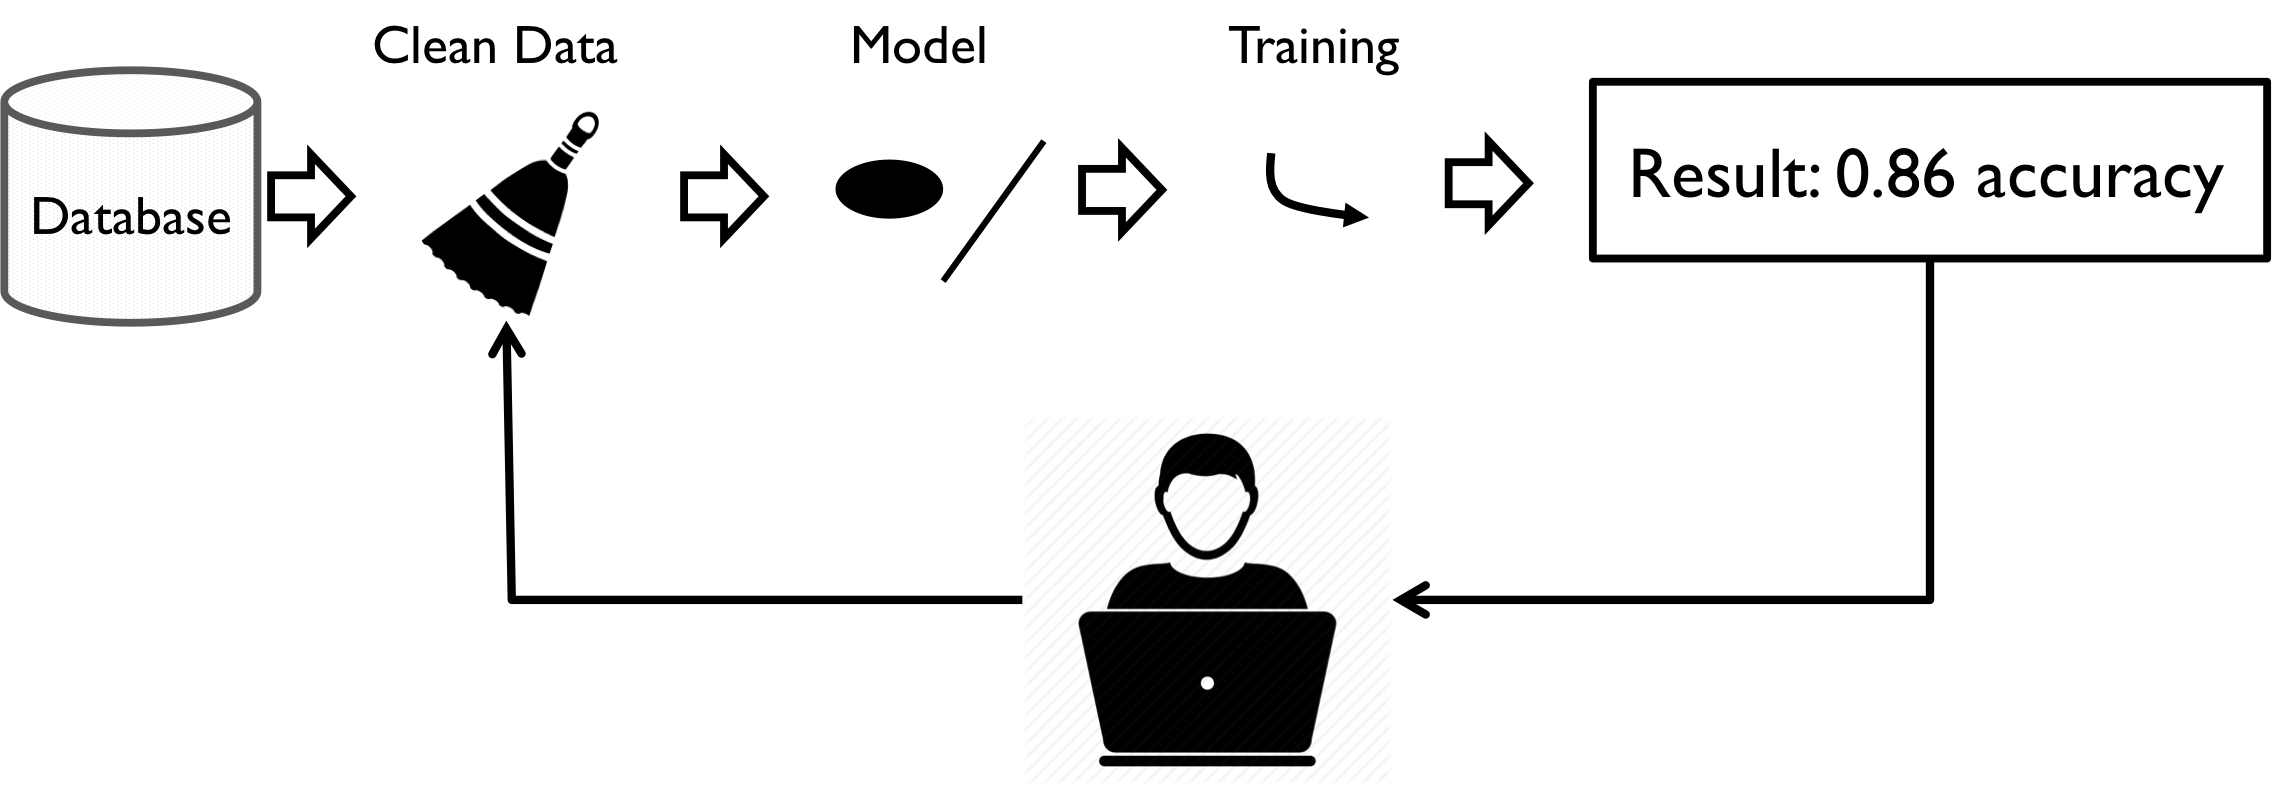
\includegraphics[width=0.8\columnwidth]{figs/workflow.png}
 \caption{Analysts often clean data interactively with data analytics; iteratively cleaning some data and re-training on a partially clean dataset to evaluate whether the cleaning was effective. It is common to use the preliminary analysis on dirty data as a guide to help identify potential errors and design repairs. \label{cartoon}}
\end{figure}

\subsection{Iteration in Model Construction}
Consider an analyst designing a classifier on the ProPublica dataset.
When she first develops her model on the dirty data, she will find that the detection rate (true positives predicted) is quite low 66\%.
To investigate why she might examine those records that are incorrectly predicted by the classifier.

Several studies have reported that this process is non-linear, iterative, and adaptive.
It is common for analysts to use the preliminary analysis on dirty data as a guide to help identify potential errors and design repairs~\cite{kandel2012}.
For example, our analyst may discover that there are numerous examples where two records are nearly identical, but one is predicted correctly, and one is incorrect, and their only difference is the \texttt{corporation} attribute: Pfizer and Pfizer Incorporated.
Upon discovering such inconsistencies, she will merge those two attribute values, re-train the model, and repeat this process (Figure \ref{cartoon}).

We define iterative data cleaning to be the process of cleaning subsets of data, evaluating preliminary results, and then cleaning more data as necessary.
\sys explores two key questions about this iterative process: (1) \emph{Correctness.} Will this clean-retrain loop converge to the intended result and (2) \emph{Efficiency.} How can we best make use of the existing data and analyst effort.

\vspace{0.5em}
\noindent \textbf{Correctness: } The straight-forward application of data cleaning is to repair the corruption in-place, and re-train the model after each repair.
However, this process has a crucial flaw, where a model is trained on a mix of clean and dirty data.
It is known that aggregates over mixtures of different populations of data can result in spurious relationships due to the well-known phenomenon called Simpson's paradox \cite{simpson1951interpretation}.
Simpson's paradox is by no means a corner case, and it has affected the validity of a number of high-profile studies~\cite{pearl2003causality}.
Figure \ref{update-arch1} illustrates a simple example where such a process can lead to unreliable results, where artificial trends introduced by the mixture can be confused for the effects of data cleaning.
The consequence is that after applying a data cleaning operation on a subset of data the analyst cannot be sure if it makes the model more or less accurate.
\emph{\sys provides an update algorithm with a monotone convergence guarantee where more cleaning is expected to lead to a more accurate result.}

\vspace{0.5em}
\noindent \textbf{Efficiency: } One could alternatively avoid the mixing problem by taking a small sample of data up-front, perfectly cleaning it, and then training a model.
This approach is similar to SampleClean \cite{wang1999sample}, which was proposed to approximate the results of aggregate queries by applying them to a clean sample of data.
However, high-dimensional models are highly sensitive to sample size, and it is not uncommon to have models whose training data complexity is exponential in the dimensionality (i.e., the curse of dimensionality).
Figure \ref{update-arch1}c illustrates that, even in two dimensions, models trained from small samples can be as incorrect as the mixing solution described before.
Sampling further as a problem of scarcity, where errors that are rare may not show up in the sample.
\emph{\sys uses a model trained on the dirty data as an initialization and uses this model as guide to identify future data to clean.}

\vspace{0.5em}
\noindent \textbf{Comparison to Active Learning: } In spirit, \sys is similar to Active Learning~\cite{DBLP:journals/pvldb/YakoutENOI11,gokhale2014corleone} as both seek to reduce the number of queries to an analyst or a crowd.
However, the two approaches consider different problems.
Active Learning considers the problem of selecting the most informative unlabeled examples to label in partially labeled static data.
Active Learning iteratively queries new examples to label and integrates those examples into the model.
In contrast, \sys studies the broader problem of prioritizing modifications to both features and labels in existing examples.

%This would be like Active Learning, where instead of unlabled data, there are inaccurate prior estimates for the labels.
%\sys reduces to a form of Expected Gradient Length Active Learning when there is no structure in the dirty data to exploit (such as completely missing attribute values).




